\section{Арбитражная стратегия}

В нашем проекте мы, конечно, не могли не попробовать одну из самых распространённых и классических стратегий высоко частотного трейдинга -- арбитраж. Идейно в этой стратегии все просто: мы смотрим на цену на одной бирже (сигнальной) и если она резко пошла вверх или вниз, то предпринимаем соответствующие действия на нашей бирже.

\subsection{Описание стратегии}
Если мы засекли быстрое и сильное изменение цены на сигнальной бирже, то выставляем рыночный ордер на нашей бирже в направлении изменения цены. Следом отправляем два ордера, которые будут фиксировать прибыль и убыток. Таким образом, если мы угадали с направлением движения цены, то у нас появляется шанс заработать. Ключевые параметры стратегии:
\begin{itemize}
\item \texttt{Profit threshold} -- от этого параметра зависит, насколько далеко от цены исполнения рыночного ордера мы будем выставлять ордер для фиксации прибыли.
\item \texttt{Loss threshold} -- аналогично предыдущему, но для фиксации убтков.
\item \texttt{Signal threshold} -- показывает, какое изменение в цене мы считаем "сильным",,если на сигнальной бирже оно было больше этого параметра, то можем фиксировать сигнал
\item \texttt{Window size} -- промежуток времени, за который мы фиксируем скачок. Если цена выросла на нужный \texttt{Signal threshold} за \texttt{Window size}, то тогда фиксируем сигнал, если цена росла дольше, чем \texttt{Window size}, то мы не считаем это за сигнал.
\item \texttt{Sec to wait} -- сколько мы держим рыночный ордер. Если по фиксирующим ордерам не прошла сделка и через \texttt{Sec to wait} секунд мы не зафиксировали ни прибыль, ни убыток, то закрываем нашу позицию новым рыночным ордером. 
\end{itemize}




\subsection{Выбор биржи и инструмента}
В мире сейчас очень много криптовалютных бирж, но самой крупной уже долгие годы остается Binance, поэтому мы решили наблюдать за ценой на ней, ведь там совершаются десятки сделок в секунду. Инструментов тоже существует бесчисленное множество, мы остановились на бессрочном фьючерсе биткоина, который торгуется в долларах. Такой выбор был продиктован следующими причинами: биткоин до сих пор остается самой популярной криптовалютой, цена на сам биткоин очень волатильна, а на его фьючерс и подавно, это дает нам возможность ловить большие скачки цены, на бирже dydx в основном представлены бессрочные фьючерсы и нам показалось логичным совершать сделки на основании информации о похожем инструменте.  


\subsection{Обнаружение скачков с помощью скользящего окна}
Одна из ключевых задач в арбитражной стратегии -- обнаружение быстрого и сильного изменения цены. Мы считаем, что цена изменилась быстро, если изменения произошли менее, чем за одну секунду (значит, Window size = 1000 миллисекунд) и сильно, если скачок цены был больше, чем на две комиссии на Binance (значит, Signal threshold = 1 + 2 * Binance Commission + eps). Чтобы обнаруживать такие события, был создан класс \href{https://github.com/dexety/dex-trading-system/blob/90a2ccd08234584b2ab9a274fe82533a55b924d9/utils/sliding_window.py#L12}{SlidingWindow}, реализующий \href{https://codeforces.com/blog/entry/71687?locale=ru}{алгоритм} поиска минимума в скользящем окне, адаптированного под наши нужды. Работает это примерно следующим образом:
\begin{itemize}
\item Мы создаем экземпляр класса SlidingWindow, с указанием размера окна в миллисекундах
\begin{verbatim}
slide = SlidinWindow(window_size)
\end{verbatim}

\item При поступлении нового трейда от вебсокета Binance/при анализе исторических данных, мы парсим данные и обновляем окно, добавляя туда новую цену и timestamp свежего трейда, метод push\_back возвращает True, если минимум или максимум был изменен и False иначе:
\begin{verbatim}
result = slide.push_back(price, timestamp)
\end{verbatim}

\item Далее мы смотрим, если отношение минимума цены к максимуму больше или равно нашего порога, то тогда считаем, что мы поймали скачок, который дальше можно как-то анализировать:
\begin{verbatim}
if result:
    max_in_window = self.slide.get_max()
    max_timestamp = self.slide.get_max_timestamp()
    min_in_window = self.slide.get_min()
    min_timestamp = self.slide.get_min_timestamp()
    if max_in_window / min_in_window >= (
        1 + self.signal_threshold):
            if max_timestamp > min_timestamp:
                return "BUY"
            elif max_timestamp < min_timestamp:
                return "SELL"
\end{verbatim}
\end{itemize}

Этот класс будет использоваться для поиска скачков на исторических данных и для их обнаружения в реальном времени в рабочем прототипе трейдера

\subsection{Анализ исторических данных, реагируем на все сигналы}
Чтобы понять, возможно ли вообще заработать, используя эту стратегию, был проведен анализ исторических данных. Данные с Binance мы брали из публичного \href{https://data.binance.vision/}{архива}, а данные с dydx собирали простеньким \href{https://github.com/dexety/dex-trading-system/blob/90a2ccd08234584b2ab9a274fe82533a55b924d9/research/ib-0002-cross-analysis/dydx_get_trades.py#L10}{скриптом}, впрочем, и в коннекторе есть для этого отдельная \href{https://github.com/dexety/dex-trading-system/blob/90a2ccd08234584b2ab9a274fe82533a55b924d9/connectors/dydx/connector.py#L158}{функция}.

\subsubsection{Class ProfitCalcualtor}
Для анализа исторических данных и подсчета прибыли был создан класс с говорящим названием \texttt{ProfitCalculator}, который позволяет нам понять, сколько мы теоретически можем заработать, используя арбитражную стратегию. При создании экземпляра этого класса ему обязательно передаются имена файлов, которые содержат исторические трейды с сигнальной биржи и трейды биржи, с которой мы торгуем. Можно также установить ключевые параметры стратегии, но они есть по умолчанию. Выглядит это так:
\begin{verbatim}
PC = ProfitCalcualtor(signal_filename, predict_filename, **params)
\end{verbatim}

\subsubsection{Сбор сигналов}
У класса \texttt{ProfitCalculator} есть метод \texttt{get\_signals}, который позволяет нам получить сигналы на основе трейдов, которые лежали в файле с именем \texttt{signal\_filename}. Мы можем сдампить сигналы, воспользовавшись соответствующими методами класса. И, конечно, визуализировать их тоже можно. То есть стандартный сценарий использования \texttt{ProfitCalculator} с целью получения сигналов такой:
\begin{verbatim}
PC.get_signals()
PC.dump_signals(signals_filename)
PC.show_signals()
\end{verbatim}

Вот пример работы метода \texttt{show\_signals}:
\begin{figure}[H]
\center{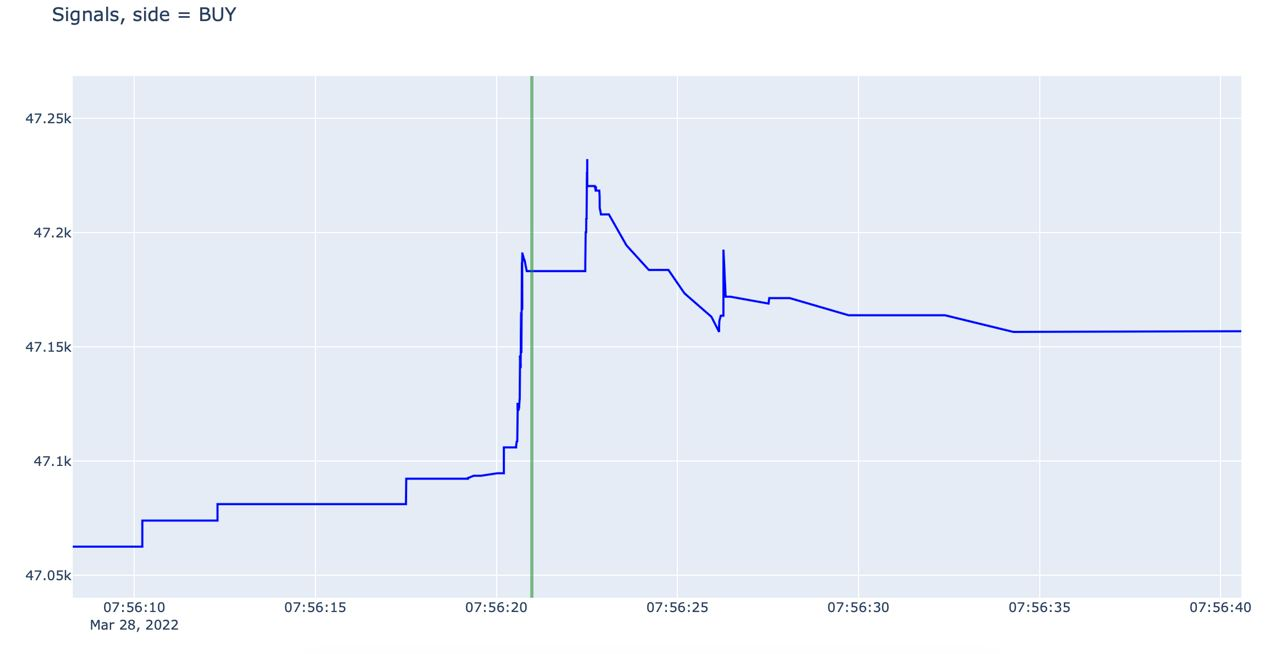
\includegraphics[scale=0.4]{img/signal.jpg}}
\caption{BUY signal example}
\label{fig:image}
\end{figure}

\subsubsection{Получение трейдов и расчет прибыли}
После того как мы получили сигналы, можно воспользоваться методам \texttt{get\_trades}, который, имитируя торговлю по арбитражной стратегии на исторических данных из файла  \texttt{predict\_filename}, сохраняет трейды. Далее можно сдампить трейды в файл с помощью метода \texttt{dump\_trades} и получить график, на котором отмечены наши сделки  помощью \texttt{show\_trades}. 
\begin{figure}[H]
\center{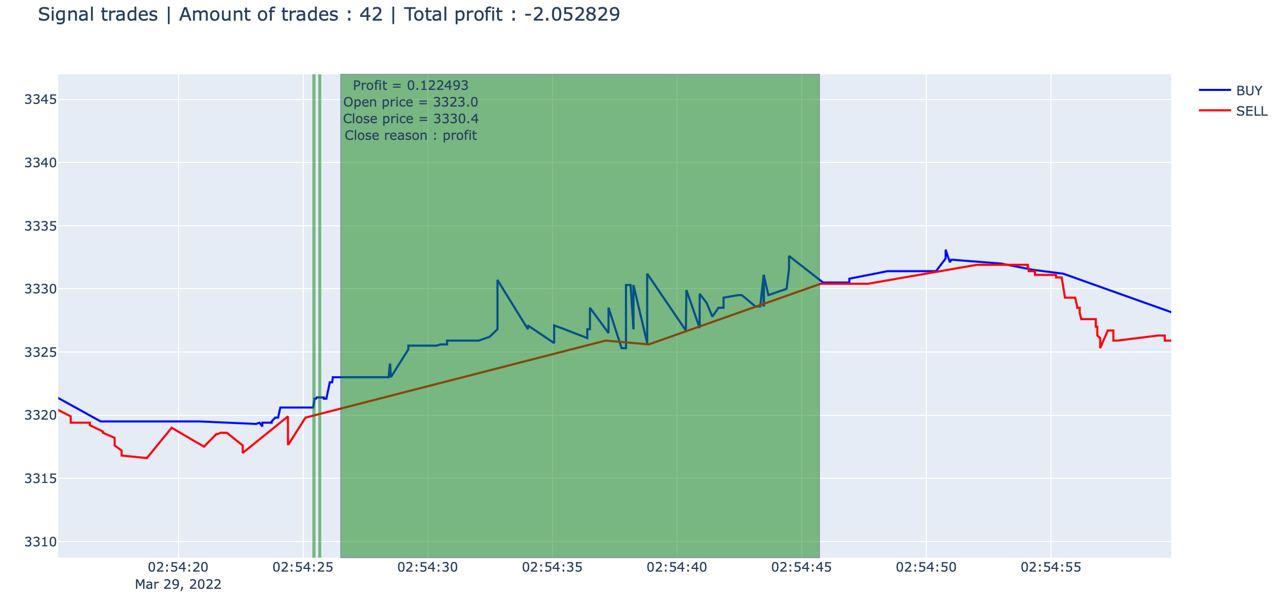
\includegraphics[scale=0.4]{img/trade.jpg}}
\caption{BUY trade example}
\label{fig:image}
\end{figure}


Теперь, когда у нас есть трейды, мы можем посчитать, на сколько процентов увеличится наш портфель. Делается это с помощью метода \texttt{get\_profit}, который возвращает нам общий профит со всех циклов открытия и закрытия позиций и список профитов для каждого из них по отдельности. Вот таблица суммарных профитов за несколько месяцев:

\begin{table}[h]
    \centering
    \begin{tabular}[t]{ | l | l | l | l | l | }
    \hline
    Dec & Jan & Feb & Mar & Apr \\ \hline
    -30.84 & 6.96 & -5.26 & -16.49 & -5.38 \\
    \hline
    \end{tabular}
    \label{table:satellites}
\end{table}

Эти значения были получены при фиксированных ключевых параметрах на весь месяц. Понятно, что можно с ними немного поиграться с целью увеличения профита, но это не дает больших результатов. Сколько бы мы не экспериментировали с ними, картина остается примерно такой же: в декабре/январе мы что-то зарабатываем, а дальше все очень плохо.







\subsection{Анализ исторических данных, попытка отсеять плохие сигналы}
Как видно из таблицы выше, ситуация скорее печальная, чем радостная. Есть несколько аномальных месяцев, которые принесли бы нам прибыль, но большинство из них все-таки были убыточными. Мы теряем много денег, когда реагируем на плохие сигналы и зарабатываем недостаточно, когда реагируем на хорошие, но выставляем плохие трешхолды. Есть два очевидных пути улучшения нашей стратегии: научиться не реагировать на плохие сигналы, либо уметь подбирать ключевые параметры стратегии для каждого сигнала по отдельности. Поговорим здесь о первом варианте (спойлер: даже он не работает).

\subsubsection{Сбор фичей}
Нам нужно выделить какие-то фичи, по которым мы будем предсказывать, будет ли сигнал прибыльным или нет. Их должно быть удобно собирать, они должны отражать фундаментальные характеристики нашего скачка. Мы выделили следующие признаки:

\begin{itemize}
\item \texttt{Average quantity} -- средняя цена объема сделки в окне.
\item \texttt{Max quantity} -- максимальная цена объема сделки в окне.
\item \texttt{Stdev price} -- стандартное отклонение цены в окне.
\item \texttt{Stdev quantity} -- стандартное отклонение объема в окне.
\item \texttt{Trades frequency} -- частота трейдов в окне.
\item \texttt{Jump value} -- величина прыжка: во сколько раз изменилась цена.
\item \texttt{Jump time length} -- длина прыжка: сколько миллисекунд потребовалось, чтобы достичь \texttt{Jump value}.
\end{itemize}

Все эти признаки легко собирать с помощью стандартного питоновского пакета \texttt{statistics}, добавив еще одно скользящее окно, отслеживающее объем трейдов, вместо их цены. Теперь метод \texttt{get\_signals} будет не только находить сигналы, но и собирать фичи к каждому из них.

\subsubsection{Узнаем, был ли сигнал теоретически прибыльным}
Для этого мы будем идти на 20 секунд вперед от времени сделки по рыночному ордеру, который мы отправили после получения сигнала, и если отношение цены хотя бы одного из трейдов за эти 20 секунд к цене рыночного была \texttt{> 1 + dydx\_commission}, то это значит, что мы могли заработать, отреагировав на этот сигнал. 

Еще по дороге будем собирать наилучшие ключевые параметры стратегии для данного сигнала: какой максимальный \texttt{Profit threshold} мы могли выставить, чтобы заработать как можно больше, какой должен был быть \texttt{Profit threshold}, чтобы не закрыться по нему, зафиксировав прибыль и т.п. Делается это просто, надо всего лишь найти минимальную/максимальную цену на окне в 20 секунд, которые мы анализируем и посчитать отношение цен.

\subsubsection{Пытаемся отличить плохие сигналы от хороших}
        Теперь у нас есть матрица вида

\begin{table}[h]
    \centering
    \begin{tabular}[t]{ | l | l | l | l | }
    \hline
    Average quantity & Max quantity & ... & Has profit \\ \hline
    100 & 1000 & ... & 1 \\
    ... & ... & ... & 0 \\
    ... & ... & ... & ... \\
    \hline
    \end{tabular}
    \label{table:satellites}
\end{table}

И мы можем попробовать поприменять к этим данным различные модели классификации, чтобы научиться отличать успешные сигналы. Но для начала посмотрим на совместное распределение фичей. Может удастся увидеть какую-то структуру в данных. 

\begin{figure}[H]
\center{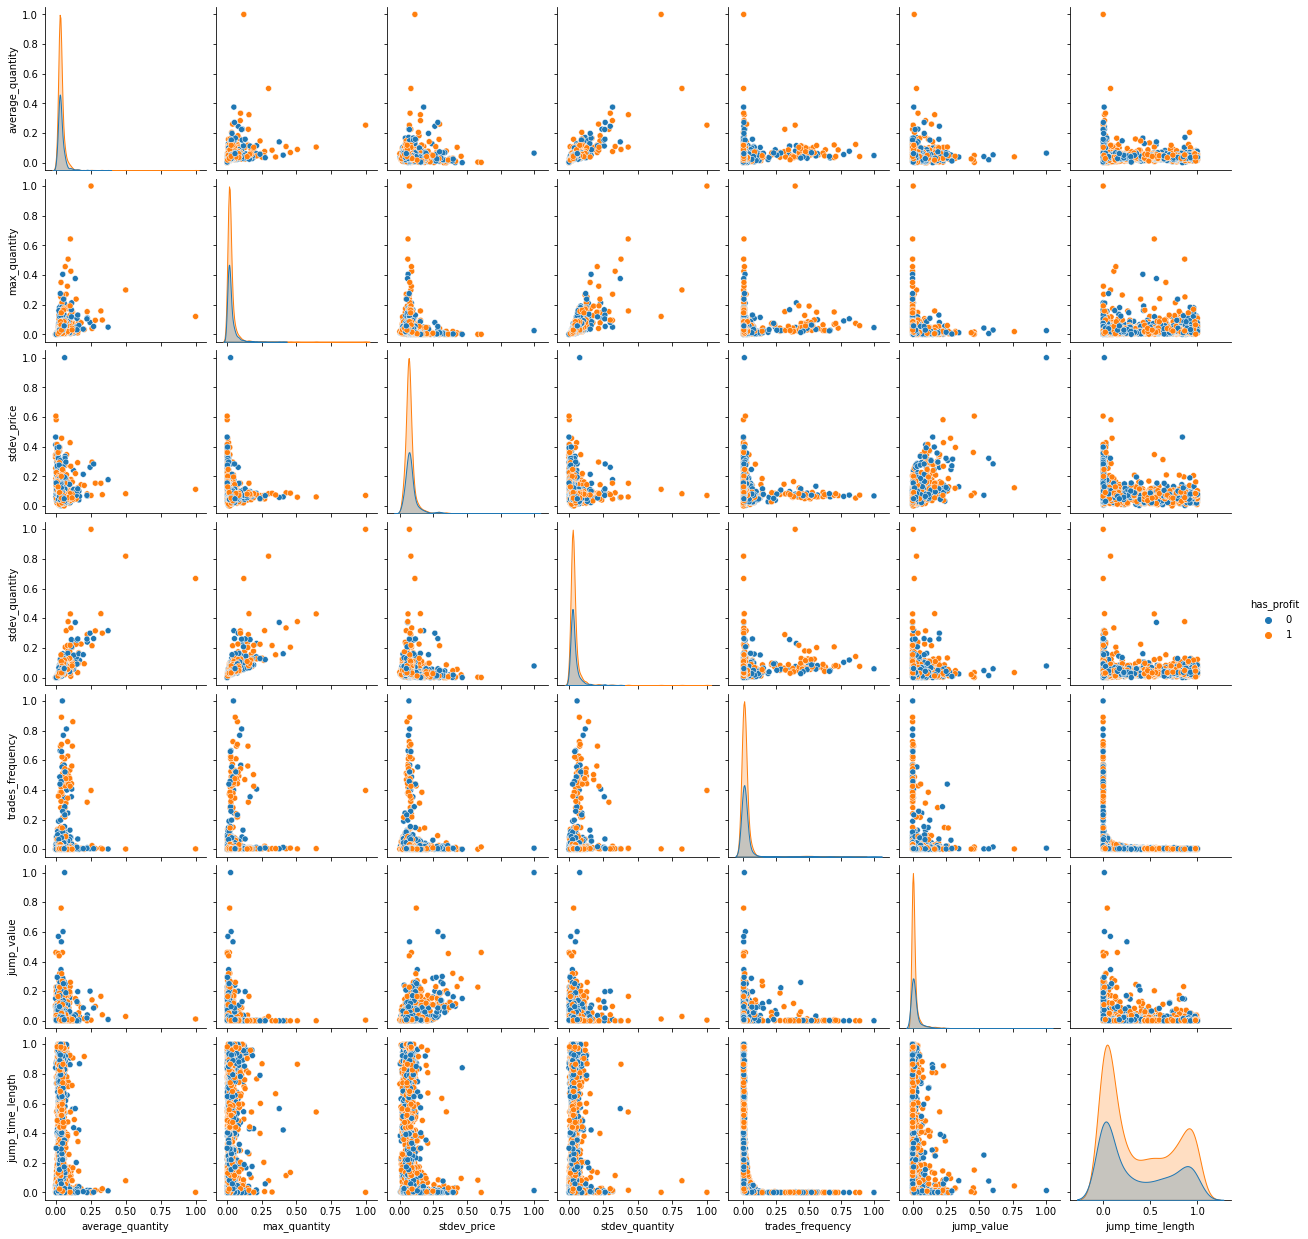
\includegraphics[scale=0.4]{img/features.png}}
\caption{Feature's distribution}
\label{fig:image}
\end{figure}

Видно, что классы очень плохо отделяются, все перемешано, шансов на хорошую классификацию очень мало. Но мы попробуем (но ничего не получиться).

\begin{itemize}
\item \textbf{Решающие деревья}

Пользуемся \texttt{DecisionTreeClassifier} из \texttt{sklearn}. Для хорошей интерпретируемости ограничим глубину дерева одним уровнем. Это даст нам понимание, какой самый значимый признак выделил классификатор.
\begin{verbatim}
from sklearn.tree import DecisionTreeClassifier
model = DecisionTreeClassifier(max_depth=1)
model.fit(X_train, Y_train_has_profit)
model.score(X_test, Y_test_has_profit)
\end{verbatim}

Результаты не очень хорошие: средняя точность составляет всего 69\%. Посмотрим на визуализацию нашего небольшого дерева:
\begin{figure}[H]
\center{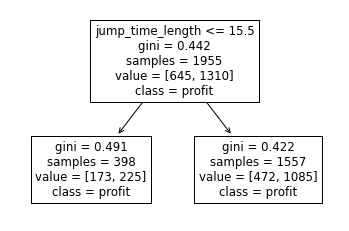
\includegraphics[]{img/tree1.png}}
\caption{Decision Tree}
\label{fig:image}
\end{figure}

Видно, что gini-коэффициент в каждой вершине довольно близок к 0.5, это означает, что данный признак плохо разделяет классы. В каждой вершине находится много сигналов обоих типов. Общее число успешных сигналов во всем нашем датасете составляет где-то 66\%. Если мы будем игнорировать все сигналы,  \texttt{Jump time length} которых меньше 100мс, то можем повысить долю успешных сигналов до 68\%:

\begin{verbatim}
>>> print(f"Было: {df_total[df_total.has_profit == 1].shape[0] 
                                                / df_total.shape[0]}")
Было: 0.6617752326413744
>>> df_total = df_total[df_total.jump_time_length > 100]
>>> print(f"Стало: {df_total[df_total.has_profit == 1].shape[0] 
                                                / df_total.shape[0]}")
Стало: 0.6815804764671702
\end{verbatim}

Можно еще раз повторить процедуру с DecisionTreeClassifier, но уже с отфильтрованным датасетом, получим такую картинку:
\begin{figure}[H]
\center{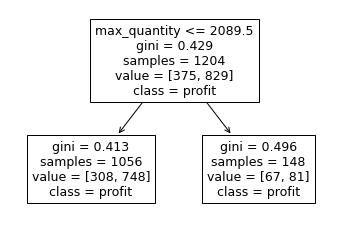
\includegraphics[]{img/tree2.png}}
\caption{Decision Tree}
\label{fig:image}
\end{figure}

Ну тоже, мягко говоря, не очень получается, но давайте опять отфильтруем датасет по этому признаку и посмотрим, возросла ли доля хороших сигналов:
\begin{verbatim}
>>> print(f"Было: {df_total[df_total.has_profit == 1].shape[0] 
                                                / df_total.shape[0]}")
Было: 0.6815804764671702
>>> df_total = df_total[df_total.max_quantity <= 2100]
>>> print(f"Стало: {df_total[df_total.has_profit == 1].shape[0] 
                                                / df_total.shape[0]}")
Стало: 0.6950732356857523
\end{verbatim}

Ну опять как-то не радостно. Можем теперь посчитать профит на разных месяцах, отсекая сигналы, у которых \texttt{Jump time length} < 100 и \texttt{Max quantity} > 2100. Получим следующие профиты:

\begin{table}[h]
    \centering
    \begin{tabular}[t]{ | l | l | l | l | l | }
    \hline
    Dec & Jan & Feb & Mar & Apr \\ \hline
    -29.29 & 4.885 & -2.57 & -6.85 & -3.15 \\
    \hline
    \end{tabular}
    \label{table:satellites}
\end{table}


Ситуация практически не изменилась, где-то улучшилась, а где-то ухудшилась, а мы ведь так старались! 

\item \textbf{Другие модели}

Мы также попробовали другие модели бинарной классификации: логистическая регрессия, решающие деревья с градиентным бустингом, даже какие-то совсем базовые нейросети. Но ничего не дает внушительного результата, который бы позволял нам зарабатывть больше.
\end{itemize}

Что касается попытки предсказывать ключевые параметры стратегии, то она была обречена на провал, ведь если задуматься, одной из характеристик модели, которая бы предсказывала параметры, как раз является умение отличить плохой сигнал от хорошего, а мы это сами не смогли сделать. Попробовали разные виды линейных регрессий с регуляризацией, различные регрессоры, основанные на решающих деревьях, но все это не принесло никаких хороших результатов. Очень жаль! 

Но мы все-таки решили написать трейдер, который реализует эту стратегию, и об этом следующая часть.